\section{Results \& Verification}
\label{sec:results}
% read revit file and 
\subsection*{Input Data and Experiment setting}
The Input Data will be BIM model in Revit format, which is a hospital. We assume that the renovation activity is to install 
a new air conditioning system in the hospital. Here is the BIM model of the hospital (Figure \ref{fig:hospital}).
\begin{figure}
    \centering
    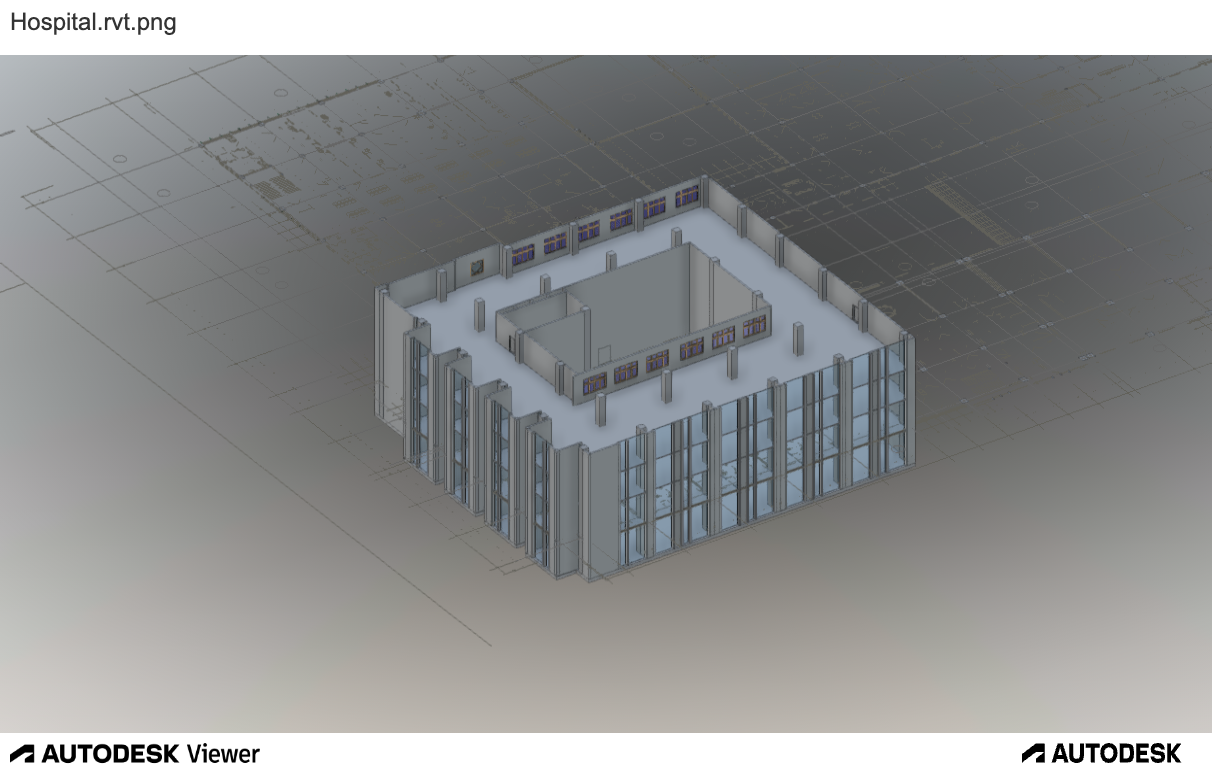
\includegraphics[width=0.5\textwidth]{figures/Hospital.rvt.png}
    \caption{Hospital BIM model}
    \label{fig:hospital}
\end{figure}

The LLM model we choose is OpenAI's GPT-4o. We call the API of GPT-4o in Python environment to build our safety management system.
The platform of Graph Database we choose is Neo4j. We use the Neo4j Desktop to build the graph database and query the graph database.

\subsection{The Final Interactive Interface}
The final interactive interface is a QA system, which is run on command line mode. It could be transfer to a web-based platform
or Autodest Revit. But for the convenience of the experiment, we only implement the command line mode.

% the result of the system is still undefine,
The dialogue between the user and the system is shown in the Figure %\ref{fig:dialogue}.
% \begin{figure}
%     \centering
%     \includegraphics[width=0.5\textwidth]{figures/dialogue.png}
%     \caption{Dialogue between the user and the system}
%     \label{fig:dialogue}
% \end{figure}
The generated report is listed in the Table.
% \begin{table}
%     \centering
%     \label{tab:report}
%     \begin{tabular}{ccccc}`'
%         \hline
%         \textbf{Involved Activities} & \textbf{Risks} & \textbf{Risk Frequency} & \textbf{Related Regulation} & \textbf{} \\
%         \hline
        
%         \hline
%     \end{tabular}
%     \caption{Generated Report}
%     \label{tab:report}
% \end{table}




